\chapter{Polimorfismo}

Un método polimórfico es aquel que tiene un comportamiento diferente dependiendo del contexto en el que se realiza la llamada.

Es decir, es un método que ha sido redefinido en varias clases dependiend del uso que le queramos dar.

Tenemos un polimorfísmo en tiempo de compilación, polimorfísmo de ejecución y polimorfísmo paramétrico.

\section{Polimorfismo en tiempo de compilación}
Lo encontramos en la \textbf{sobrecarga de operadores} y en la \textbf{programación genérica} al hacer uso de \textit{templates}.

En la sobrecarga cambia el contexto mediante la lista de parámetros que recibe el método.
\begin{itemize}
	\item \textbf{Conversiones estándar} → Se convierte un tipo de dato a otro completamente diferente, por ejemplo de \texttt{int} a \texttt{double}.
	\begin{itemize}
		\item Encontramos las promociones donde se convierte un tipo a uno con mayor rango (siempre del mismo tipo), por ejemplo de \texttt{int} a \texttt{long}, pero no un \texttt{int} a \texttt{double}. 
	\end{itemize}	
	\item \textbf{Conversiones definidas por el usuario} → Se define mediante constructores de conversión y operadores de conversión, preferiblemente el segundo. Solo intenta una conversión implícita, si se puede realizar bien, si no lanzará un error.
	\item \textbf{Coincidencia con elipsis} → Si la lista de parámetros la terminamos con puntos suspensivos (…). 
\end{itemize}
En las plantillas el compilador mira los tipos de los parámetros que recibe la clase.

\section{Polimorfismo en tiempo de ejecución}
\begin{figure}[h]
	\begin{center}
		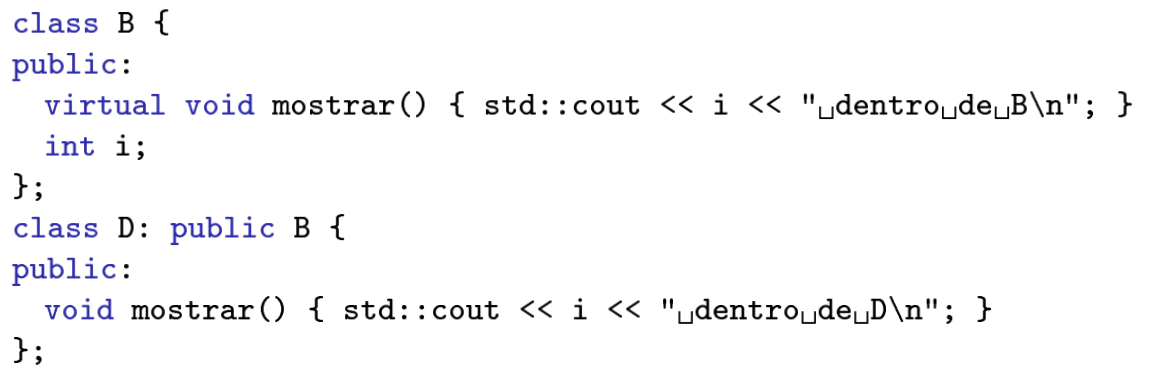
\includegraphics[width=\textwidth]{Imagenes/pol1.png}
	\end{center}
\end{figure}
La clase B es una clase \textbf{polimorfica} ya que tiene un método definido como \texttt {virtual}.

La clase D tendrá dos miembros → el atributo \texttt{int i} y el método \texttt{mostrar()} , ya que hemos definido el método `\texttt{mostrar()} ) de la clase B como virtual, es decir el compilador sabe que ese método es polimórfico y por tanto se redefinirla en la clase derivada.

Esto sucede siempre y cuando la clase derivada tendrá un método con el mismo nombre y ese se defina como `virtual` en la clase base.
\begin{figure}[h]
	\begin{center}
		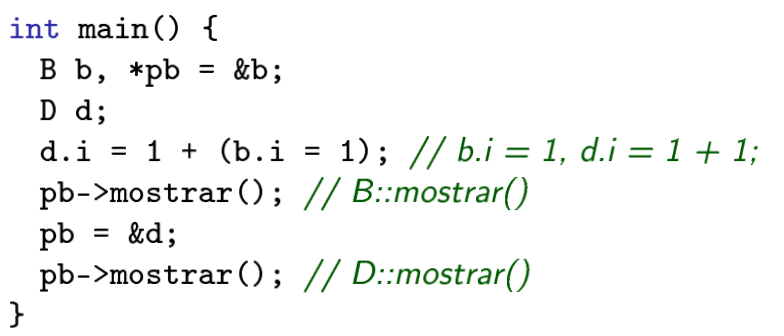
\includegraphics[width=\textwidth]{Imagenes/pol2.png}
	\end{center}
\end{figure}

En el caso de \texttt{pb->mostrar()} ya no nos fijamos en el tipo del puntero, si no en el tipo del objeto, en este caso B. 

En \texttt{pb = \&d} y \texttt{pb->mostrar()} accederá al método mostrar de la clase D, ya que el objeto al que apunta es de tipo D.

Todo esto sucede ya que hemos declarado como virtual el método mostrar, si no fuera así se llamaría siempre al método que concuerde con el tipo del puntero, en este caso el de la clase B.

\subsection{Ejemplo 1 - Polimorfismo en tiempo de ejecución}

\begin{figure}[h]
	\begin{minipage}{0.55\textwidth}
		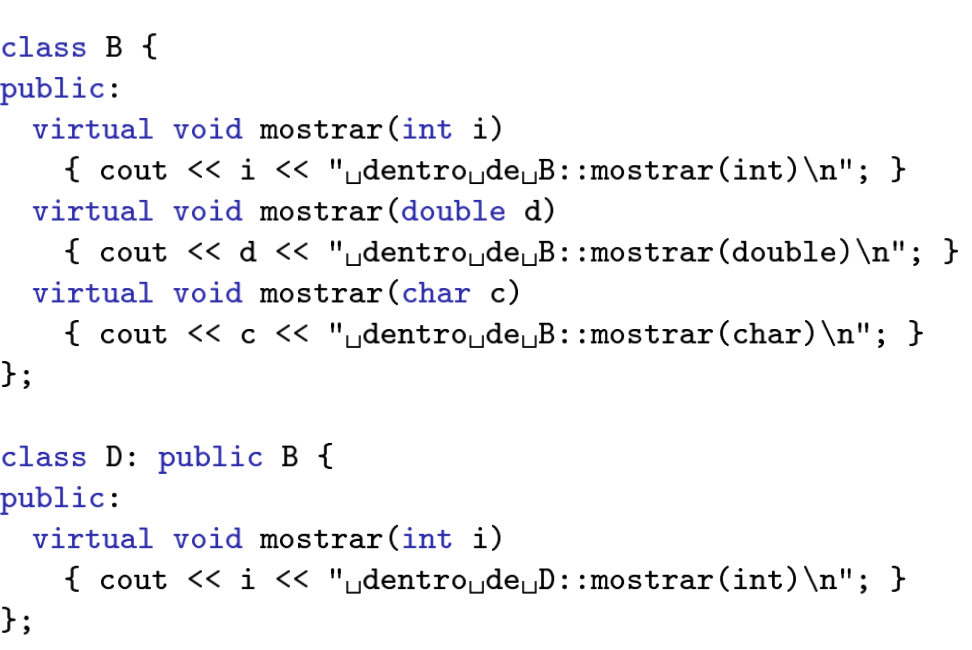
\includegraphics[width=\textwidth]{Imagenes/pol3.png}
		\caption{Cabeceras}
	\end{minipage}
	\hfill
	\begin{minipage}{0.45\textwidth}
		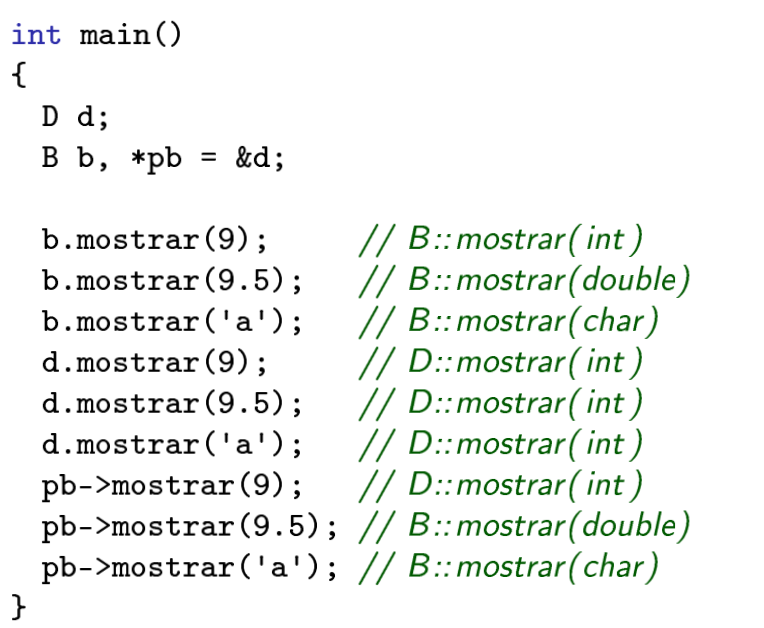
\includegraphics[width=\textwidth]{Imagenes/pol4.png}
		\caption{Código de prueba}
	\end{minipage}
\end{figure}

En este ejemplo, la clase D tiene 3 métodos dos heredados por la clase B (los que recibe un double y char) respectivamente y uno que ha sido redefinido (el que recibe un int).

Como los métodos mostrar que reciben que reciben parámetros \texttt{double}  y \texttt{char} solamente se pueden acceder a ellos cuando lo llamamos mediante un objeto de la clase B.

Si hacemos \texttt{d.mostrar('a');} nos mostrará \texttt{D::mostrar(int)}, pero si hacemos \texttt{b.mostrar(’a’);} nos mostrará \texttt{B::mostrar(char);} 

Si lo hacemos mediante punteros, se realiza un enlace dinámico que hace que comprueba el tipo del objeto de la clase, dependiendo de ese tipo llamará a un método mostrar.

Vemos que \texttt{pb} apunta a un objeto de la clase D, pero a la hora de pasarle los parámetros comprueba que método de ese objeto se corresponde a la lista de parámetros, por tanto, si se le pasa un entero y este apunta a un objeto de la clase D, se usará el método mostrar de la clase derivada D, pero como este no tiene un método redefinido para \textit{double} o \textit{char}, se llamará al método mostrar correspondiente del tipo del puntero, es decir, de la clase base B.

\subsection{Ejemplo 2 - Polimorfismo en tiempo de ejecución sin interfaz}

\begin{center}
	\begin{lstlisting}[frame=single]
class Figura{
  public:
    virtual ~Figura() {};
    virtual double area()const {return 0.0;}// por omision 
};
class Rectangulo: public Figura {
  public:
    Rectangulo(double lado_1, double lado_2);
    double area() const override;
  protected:
    double lado_1, lado_2;
};
class Circulo final: public Figura {
  public:
    Circulo(double radio);
    double area() const override;
  private:
    double radio;
};		
	\end{lstlisting}
\end{center}

Como vemos, la clase Figura es una clase polimorfica, de donde se derivan varias clases (Rectágunlo y Círculo).

El método \texttt{area()} es un método polimorfico que tendrá un comportamiento diferente en cada una de las clases derivadas.

\begin{center}
	\begin{quote}
	\textbf{Si hacemos el destructor virtual nos aseguramos que se llame al destructor de la clase derivada.\\
		Siempre que tengamos una clase polimorfica, su destructor debe de ser \texttt{virtual}.}

\end{quote}
\end{center}
\newpage
\subsection{Ejemplo 2 - Polimorfismo en tiempo de ejecución con interfaz}
\begin{figure}[h]
	\begin{center}
		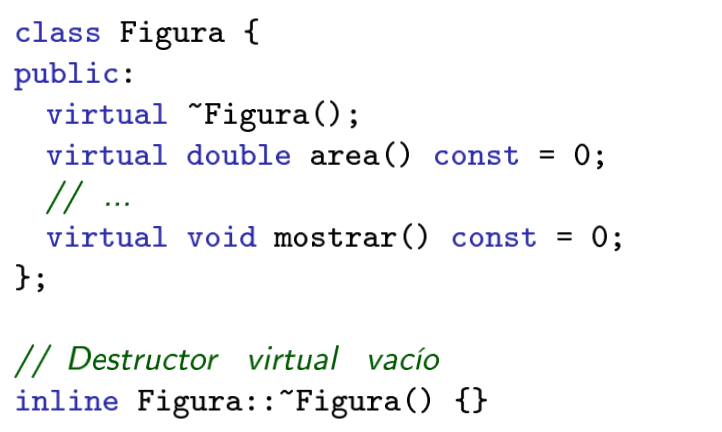
\includegraphics[width=\textwidth]{Imagenes/poli5.png}
		\caption{Definición clase Figura}
	\end{center}
\end{figure}

Convertimos la clase Figura como una clase \textbf{abstracta} haciendo que sus métodos sean \textit{virtuales puros}.

Es decir, sus métodos solo se declaran no se implementan y además no se pueden instanciar (no se pueden crear objetos de la misma), es una clase \textit{incompleta}.

\begin{figure}[h]
	\begin{minipage}{0.5\textwidth}
		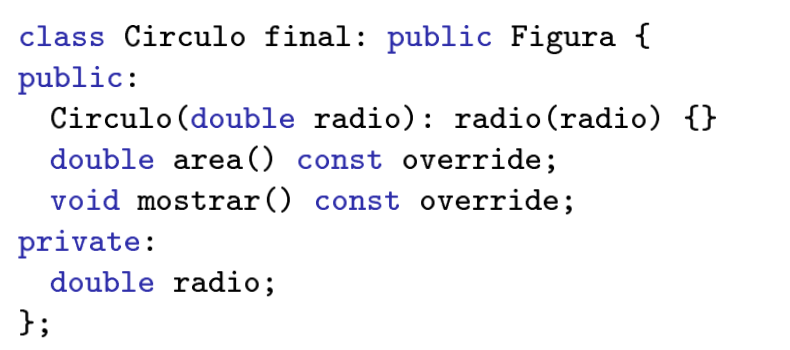
\includegraphics[width=\textwidth]{Imagenes/poli6.png}
	\end{minipage}
	\hfill
	\begin{minipage}{0.5\textwidth}
		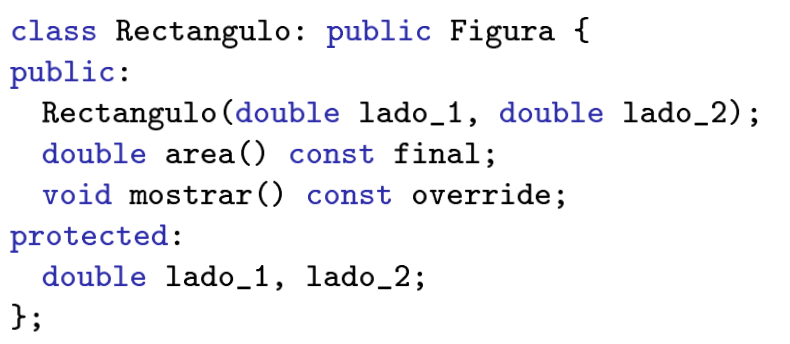
\includegraphics[width=\textwidth]{Imagenes/poli7.png}
	\end{minipage}
\end{figure}

Encontramos la \textit{keyword} \texttt{override} que le indicamos al compilador que dicho método se va a volver a implementar.

La \textit{keyword} \texttt{final} indicamos que es la versión final de la implementación de dicho método.

No podemos hacer uso de \texttt{override} y \texttt{final} a la vez ya que le estamos diciendo al compilador que se va a volver a redefinir cuando no puede ya que he hemos indicado que es la última vez que se redefine con \textit{final}.
\newpage
\begin{figure}[h]
	\begin{center}
		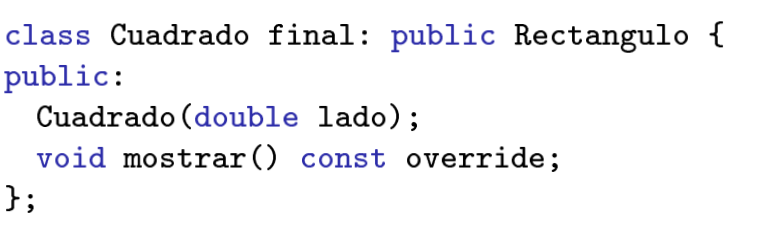
\includegraphics[width=\textwidth]{Imagenes/poli8.png}
	\end{center}
\end{figure}

Vemos que Cuadrado es una especialización de Rectángulo pero este no redefine el método \texttt{area()} debido a que se calculan igual, por eso anteriormente la definimos como final.

\section{Clases abstractas}

Son aquellas que al menos uno de sus métodos como \textbf{virtual puro}, haciendo que dicho método se pueda volver a definir en las clases derivadas de ella.

\textbf{\large{Definición de un método virtual puro:}}
\begin{center}
	\texttt{virtual void nombre\_metodo() = 0;}
\end{center}

Su destructor tiene que ser \texttt{virtual} para que se pueda llamar a los destructores de las clases derivadas con el fin de destruir el objeto creado correctamente (destructor de la misma clase del tipo de objeto).

Además con esto hacemos que se enlace en tiempo de ejecución debido a que no sabemos si vamos a tener o no objetos de las clases derivadas.

Haciendo que se llame primero al destructor de la clase derivada y luego al destructor de la clase base.


\section{Operadores de conversión}
Para poder realizar las conversiones correctamente entre la clase base y sus derivadas, es decir, para poder convertir un puntero de tipo base a uno de tipo derivado haremos uso de \texttt{dynamic\_cast} y de \texttt{typeid()}

\subsection{Operador de conversión: Dynamic\_cast}
La conversión se realiza en tiempo de ejecución a diferencia de \texttt{static\_cast} que se realiza en tiempo de compilación.

\textbf{\large Sintaxis:}
\begin{center}
	\texttt{Derivada* pd = dynamic\_cast<Derivada*>(pb)}\\
	para punteros.
	
	\texttt{Derivada\& d = dynamic\_cast<Derivada\&>(b)}\\
	para objetos.
\end{center}

Esto soluciona el peligro de realizar la conversiones explícitamente de arriba a abajo mediante \texttt{static\_cast}.

\subsubsection{Ejemplo de conversión con dynamic\_cast}

\begin{figure}[h]
	\begin{minipage}{0.5\textwidth}
		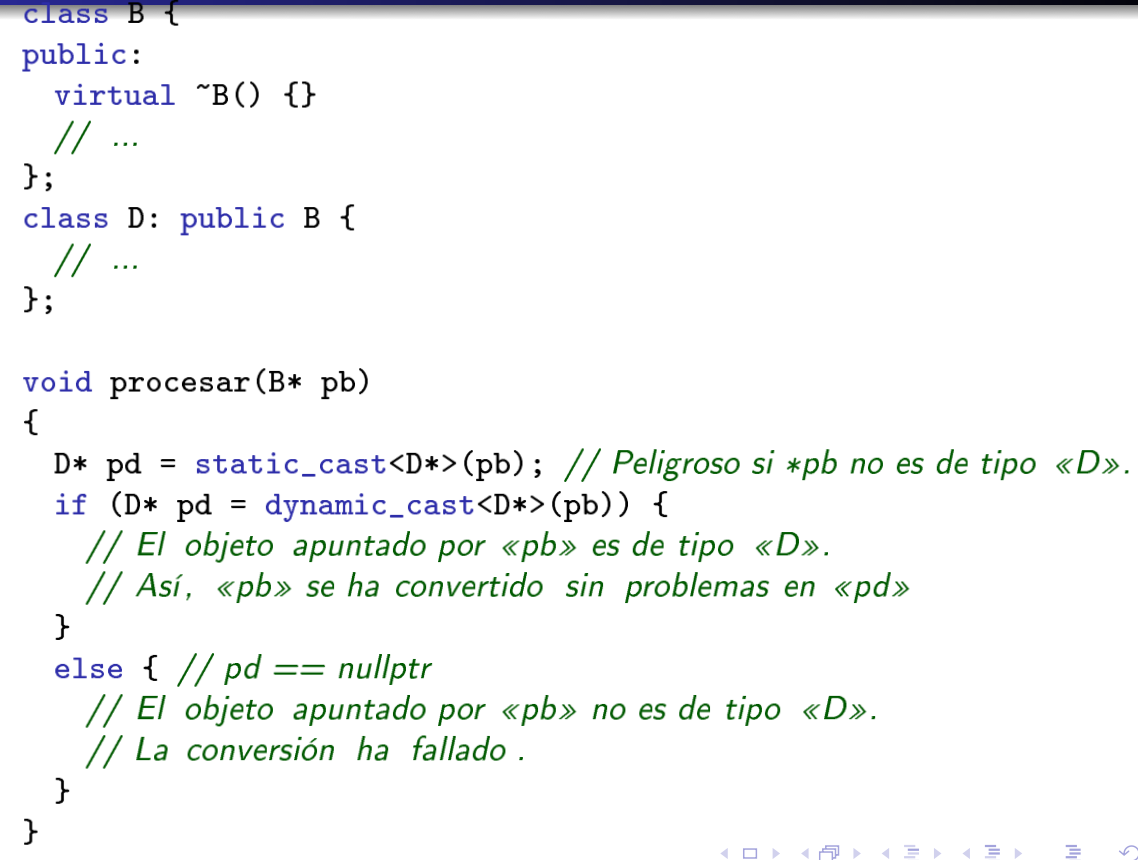
\includegraphics[width=\textwidth]{Imagenes/poli9.png}
	\end{minipage}
\hfill
	\begin{minipage}{0.5\textwidth}
		\vspace{-2cm}
		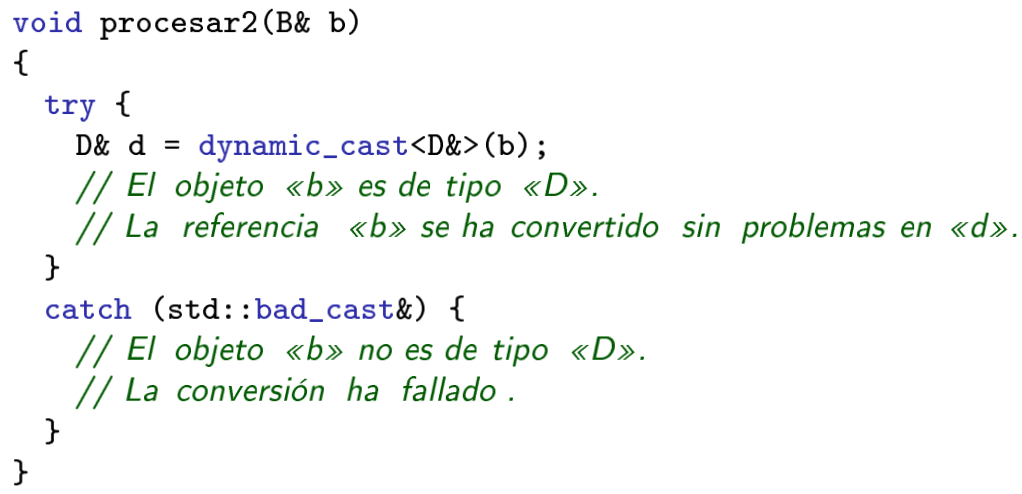
\includegraphics[width=\textwidth]{Imagenes/poli10.png}	
	\end{minipage}
\caption{Ejemplo de conversiones explicitas de un tipo base B a un tipo derivada D.}
\end{figure}

Vemos que comprueba si la conversión es correcta, si es así lo convierte a tipo indicado, si no, devuelve un puntero nulo (si es conversión entre punteros) o un \texttt{bad\_cast} (si la conversión es entre referencias), en el caso de que sea una referencia.

Cuando trabajamos con clases polimorficas es mucho más seguro trabajar con \texttt{dynamic\_cast} ya que podemos lanzar excepciones cuando la conversión no se puede realizar.

\subsection{Operador de conversión: typeid()}

Es un operador que devuelve por referencia un objeto no modificable del tipo \texttt{type\_info}.

Está declarado en la cabecera \texttt{<typeinfo>}.

\begin{figure}[h]
	\begin{center}
		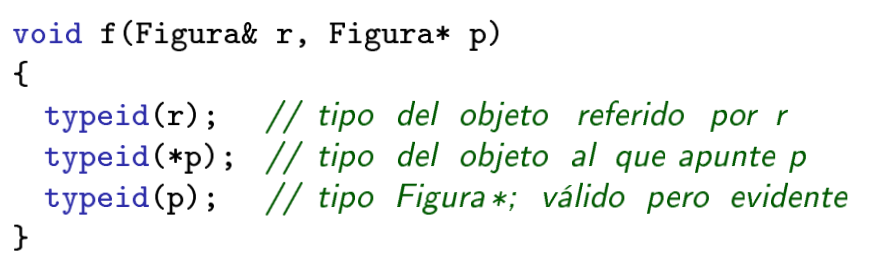
\includegraphics[width=\textwidth]{Imagenes/poli11.png}
	\end{center}
\end{figure}

Este operador si no lo almacenamos con type\_info, nos devuelve el tipo de dato al que se le pasa como parámetro.

\newpage
\section{Polimorfismo paramétrico}

\subsection{Introducción}

Vamos a hacer uso de este tipo de polimorfismo mediante las plantillas de clases (\textbf{templates}).

Se realiza en tiempo de compilación.

Podemos aplicar técnicas de programación genérica, para trabajar como tipos de datos como parámetros. Podemos definir clases donde el comportamiento de los métodos/funciones de la clase genérica dependerá del tipo de dato que se pase como parámetro.

Lo importante son los requisitos que deben de cumplir esos parámetros, es decir, encontramos precondiciones para los tipos de datos de dicha plantilla. Estas plantillas pueden recibir \textit{datos} (tipo del dato y nombre del parámetro) y \textit{tipos de datos} (\texttt{typename} o \texttt{class}).

No usamos la plantilla como tal, si no que hacemos uso de \textit{especializaciones} ó \textit{instancias} de la misma.

Los métodos de una clase genérica se implementan mediante una función genérica, para ello se pone \texttt{template <typename T>\ Clase<T>:: nombre\_metodo(parámetros)}. En este caso, incluimos el \texttt{.cpp} dentro del fichero de cabecera \texttt{.hpp} para mantener el principio de ocultación de información a la hora de instanciar plantillas.

Estas clases paramétricas las podemos relacionar con otras mediante cualquier tipo de relación vista anteriormente (asociación, composición,…).

\subsection{Deducción de parámetro}

\begin{figure}[h]
	\begin{center}
		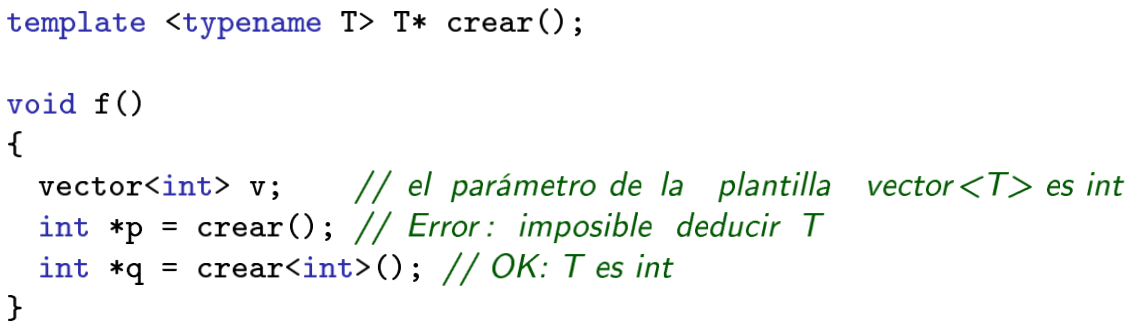
\includegraphics[width=\textwidth]{Imagenes/poli12.png}
	\end{center}
\end{figure}

El compilador mira el tipo de los parámetros reales para deducir el tipo de datos formal (T).

En algunos casos al compilador le falta información y no puede resolver el polimorfísmo paramétrico.

Vemos que en este ejemplo estamos definiendo una plantilla de función, donde el tipo de la plantilla se corresponde al tipo de los parámetros reales de la función. Si esta carece de parámetros no se podrá deducir el tipo de la plantilla.


Si el tipo de uno de los parámetros de la plantilla a función es un tipo de dato dependiente (depende del tipo de dato de la plantilla) no podemos deducir su tipo, para ello se especifica explícitamente su tipo, véase en e caso \texttt{crear<int>();}.

\subsection{Especialización}
\begin{figure}[h]
	\begin{center}
		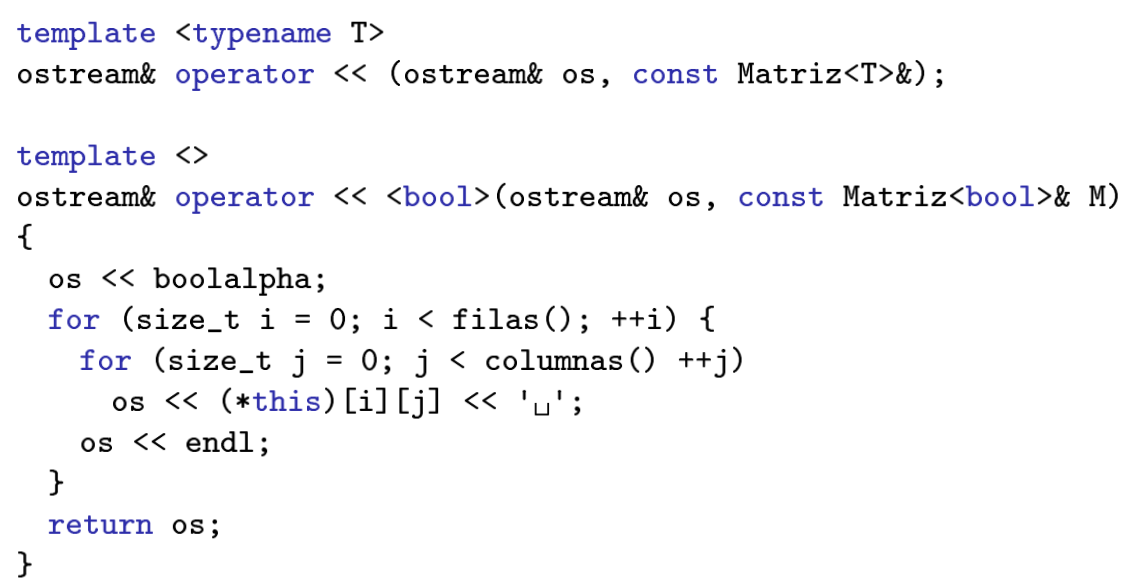
\includegraphics[width=\textwidth]{Imagenes/poli13.png}
	\end{center}
\end{figure}

Vemos que hemos especializado el operador de inserción en flujo para un tipo determinado, en este caso un booleano.

Esta es la diferencia entre polimorfísmo paramétrico y sobrecarga de operadores.

\subsection{Friend y Static en plantillas}
Los métodos que se declaran como \texttt{friend} y no se especifica el tipo, son amigas de todas las clases, pero si a esta se le especifica el tipo, solamente será amiga a la clase que concuerde con su tipo.

Al igual sucede con los atributos que se declaran como \texttt{static}.
\begin{figure}[h]
	\begin{center}
		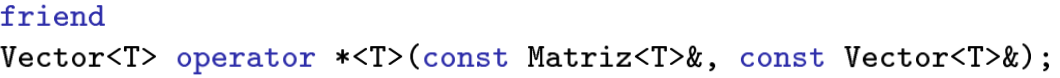
\includegraphics[width=\textwidth]{Imagenes/poli14.png}
	\end{center}
\end{figure}

Solo es amiga para la clase que concuerde con el tipo T.
















